\chapter{Results and Analysis}
\label{ch:resultsandanalysis}

This chapter presents the results of both the quantitative and qualitative analysis conducted to evaluate the impact of the mixed-reality simulation on participants’ empathy and emotional responses toward individuals with schizophrenia. It begins with a breakdown of pre-evaluation findings that show baseline attitudes and empathy. Post-evaluation results are then presented, including changes in empathy and emotional states across the full sample, as well as subgroups (group participants and individual headset users). Statistical comparisons are used to assess whether observed differences are significant. Finally, we integrate observational and verbal feedback from participants to complement and contextualize the quantitative data. This mixed-methods approach allows for a richer understanding of the simulationss effects, particularly in areas not captured by standardized measures.

\section{Pre-Evaluation Results}
The pre-evaluation phase was conducted prior to any exposure to the simulation. It served to assess baseline levels of empathy and emotional responses toward individuals with schizophrenia. We also collected information on participants' experiences with patients and with that also patients with schizophrenia, which may influence their perceptions.

\subsection{Experience with Patients and Schizophrenia}

Participants were also asked about their prior experience working with patients in general and specifically with individuals diagnosed with schizophrenia. Responses were recorded on a 5-point scale ranging from 1 (No) to 5 (Yes).


\begin{figure}[H]
    \centering
    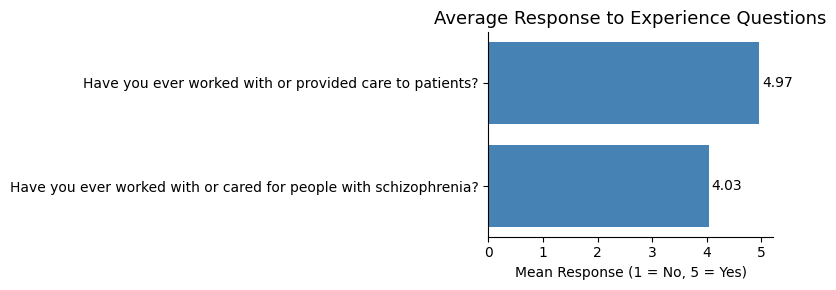
\includegraphics[width=0.7\textwidth]{../../Figures/experience-patients.png}
    \caption{Answers to questions about experience with patients and schizophrenia.}
    \label{fig:experience_patients}
\end{figure}

As shown in Figure~\ref{fig:experience_patients}, nearly all participants reported prior experience working with or caring for patients, with an average response of 4.97. However, fewer had direct experience with individuals with schizophrenia, as indicated by a lower mean score of 4.03. This suggests a general familiarity with healthcare environments, but with that not as much exposure to psychiatric conditions.

\subsection{Baseline Perceptions and Empathy}

Participants responded to a set of 13 Likert-scale items evaluating cognitive and affective components of empathy. These items were scored from 1 (Strongly Disagree) to 6 (Strongly Agree), with reverse scoring applied to negatively phrased statements.

\begin{figure}[H]
    \centering
    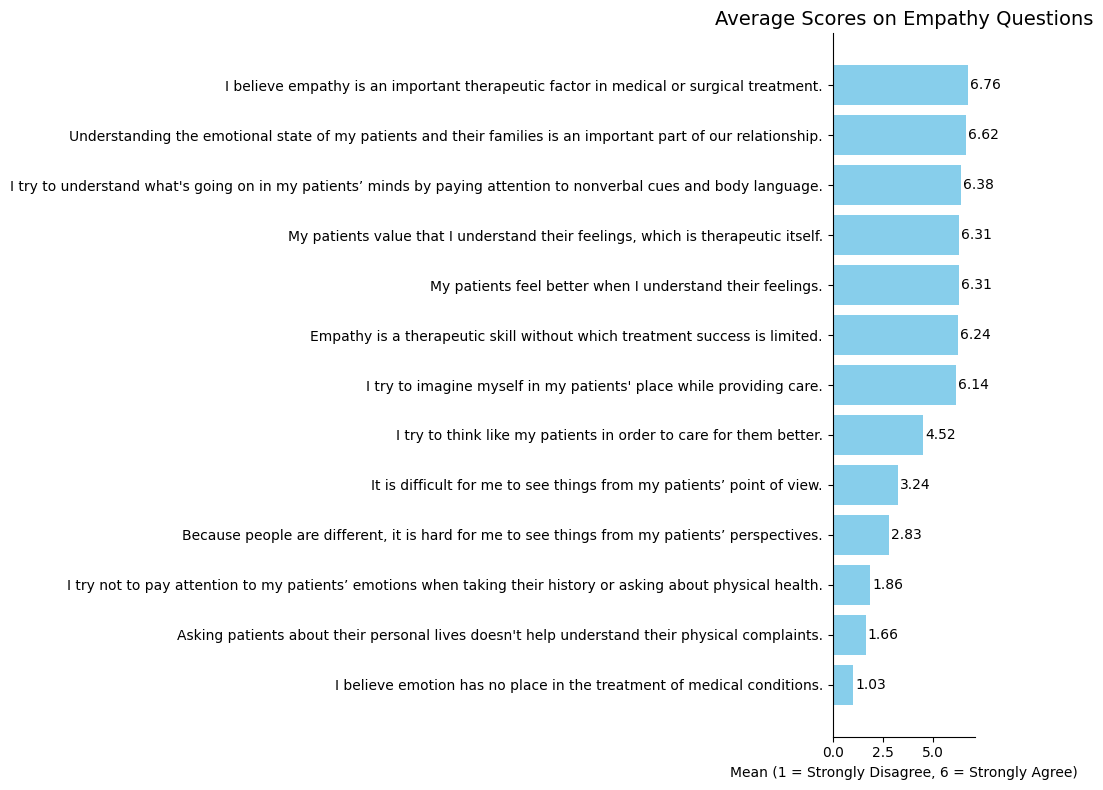
\includegraphics[width=\columnwidth]{../../Figures/avg-scores-pre.png}
    \caption{Average item-wise scores on empathy-related questions.}
    \label{fig:avg_scores_pre}
\end{figure}

Figure~\ref{fig:avg_scores_pre} shows the average scores per item. Responses were generally high for positively phrased statements (e.g., “I believe empathy is an important therapeutic factor”), indicating strong baseline attitudes in favor of empathic engagement. In contrast, negatively phrased items (e.g., “I believe emotion has no place...”) received low agreement, as expected after reverse scoring.

To explore potential variation across groups, empathy scores were also averaged by the time at which participants completed the evaluation session. These groups were constructed based on session start times.

\begin{figure}[H]
    \centering
    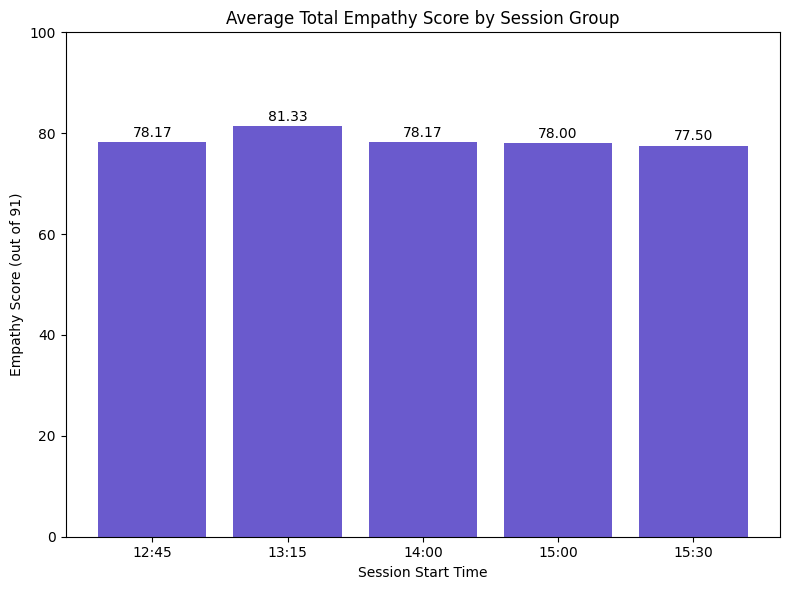
\includegraphics[width=0.75\columnwidth]{../../Figures/avg score-by-group-pre.png}
    \caption{Average total empathy score by session start group.}
    \label{fig:group_scores_pre}
\end{figure}

As shown in Figure~\ref{fig:group_scores_pre}, total empathy scores were relatively consistent across session groups. The highest group average (81.33) was observed for the 13:15 session, though variation across all time slots remained modest (range: 77.50–81.33). This suggests time-of-day or group assignment had minimal influence on baseline empathy.

Participants also rated how strongly they associated various emotions with thinking about individuals with schizophrenia, on a scale from 1 (Not at all) to 5 (Extremely).

\begin{figure}[htbp]
    \centering
    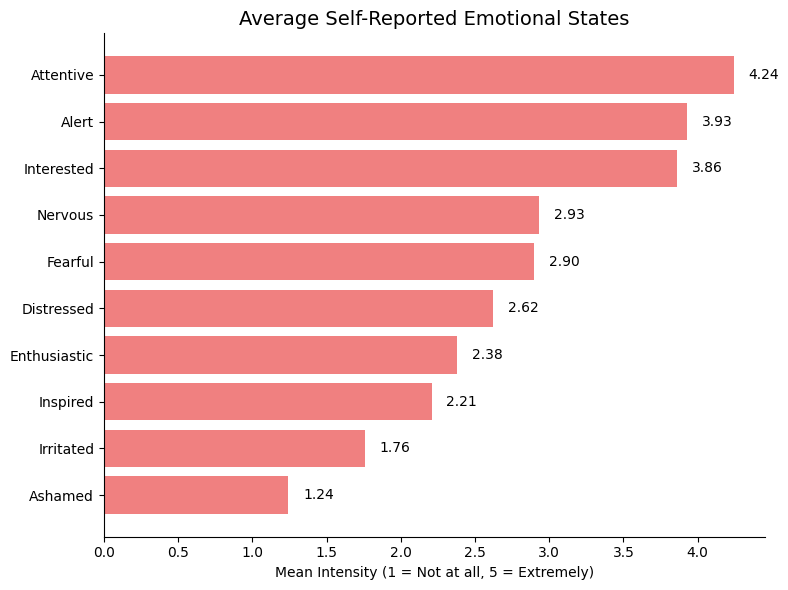
\includegraphics[width=0.7\columnwidth]{../../Figures/avg-emotions-pre.png}
    \caption{Average self-reported emotional intensity associated with thinking about people with schizophrenia.}
    \label{fig:avg_emotions_pre}
\end{figure}

Figure~\ref{fig:avg_emotions_pre} presents the average self-reported intensities for each emotion. “Attentive,” “Alert,” and “Interested” ranked highest, indicating cognitive engagement. Negative emotions such as “Ashamed” and “Irritated” were reported with relatively low intensity, suggesting a limited baseline presence of stigmatizing emotional responses.

\begin{figure}[H]
    \centering
    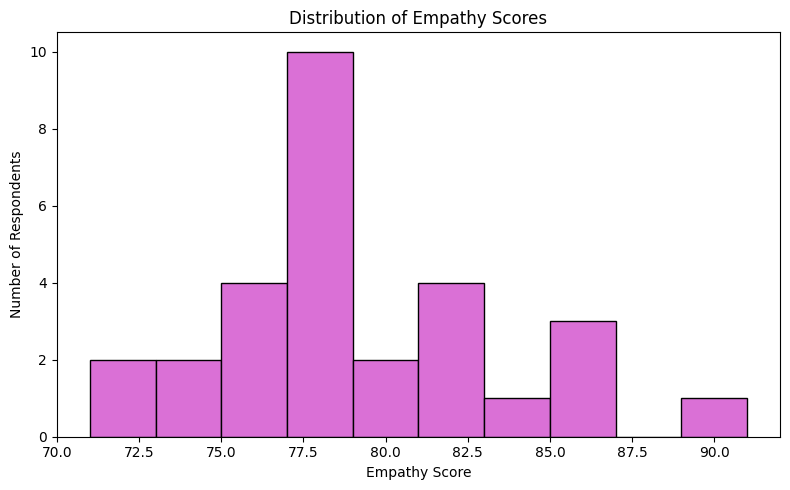
\includegraphics[width=0.75\textwidth]{../../Figures/avg-scores-summary-pre.png}
    \caption{Distribution of total empathy scores among participants.}
    \label{fig:score_distribution_pre}
\end{figure}

Finally, Figure~\ref{fig:score_distribution_pre} displays the distribution of total empathy scores. The majority of participants scored between 75 and 85 out of a maximum of 91, further confirming the high initial level of empathy among the sample.

These baseline findings establish that participants entered the intervention phase with generally high empathy and cognitive openness. This may present a ceiling effect, potentially limiting the observable shift in post-intervention scores.

\section{Post-Evaluation Results}

Following participation in the simulation, participants completed a post-evaluation survey that assessed both their emotional responses and empathy levels, which features the same question set as the pre-evaluation. These include the Jefferson Scale of Empathy (JSE) \cite{Hojat2002} to assess baseline and post-simulation empathy levels, and the Brief Positive and Negative Affect Schedule (B-PANAS) \cite{Boiroux2024} to measure emotional responses and perceptions toward individuals with schizophrenia. This section presents the results for the full sample as well as two subgroups: those who participated in a group setting and those who experienced the mixed-reality (MR) simulation individually using the headset.

Participants were asked to rate the intensity of various emotional states they experienced when thinking about individuals with schizophrenia. These ratings were provided on a 5-point scale ranging from 1 (Not at all) to 5 (Extremely).

\begin{figure}[H]
    \centering
    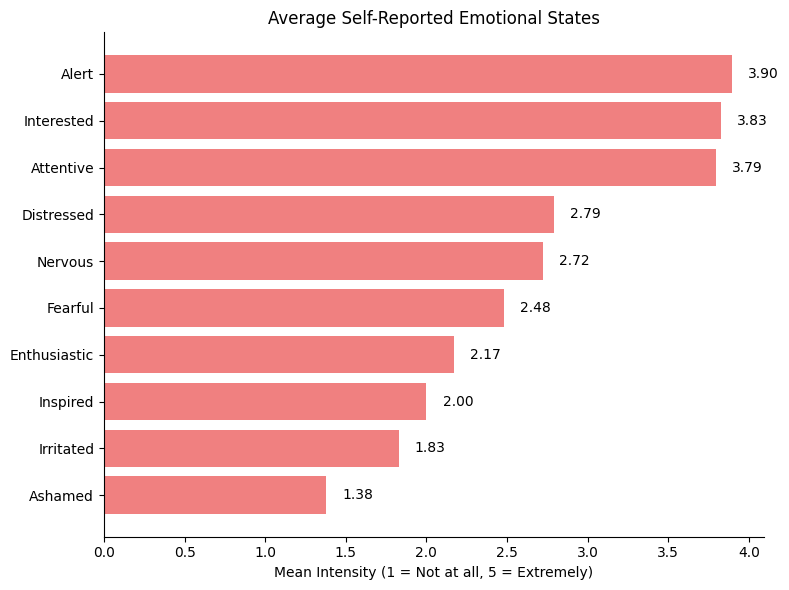
\includegraphics[width=0.75\textwidth]{../../Figures/emotional-post-all.png}
    \caption{Average self-reported emotional states (all participants).}
    \label{fig:emotional_post_all}
\end{figure}

As shown in Figure~\ref{fig:emotional_post_all}, the most intense emotions reported across all participants were \textit{Alert}, \textit{Interested}, and \textit{Attentive}, suggesting a heightened level of engagement and focus during or after the simulation. Emotions such as \textit{Ashamed}, \textit{Irritated}, and \textit{Inspired} were rated much lower, indicating that negative or affectively charged responses were less commonly experienced.

\subsection{Group Participants}

Participants who took part in the simulation in a group setting (e.g., without MR headset) reported emotional responses that were broadly similar to the overall sample. However, their average emotional intensity was slightly higher on items related to awareness and cognitive involvement.

\begin{figure}[H]
    \centering
    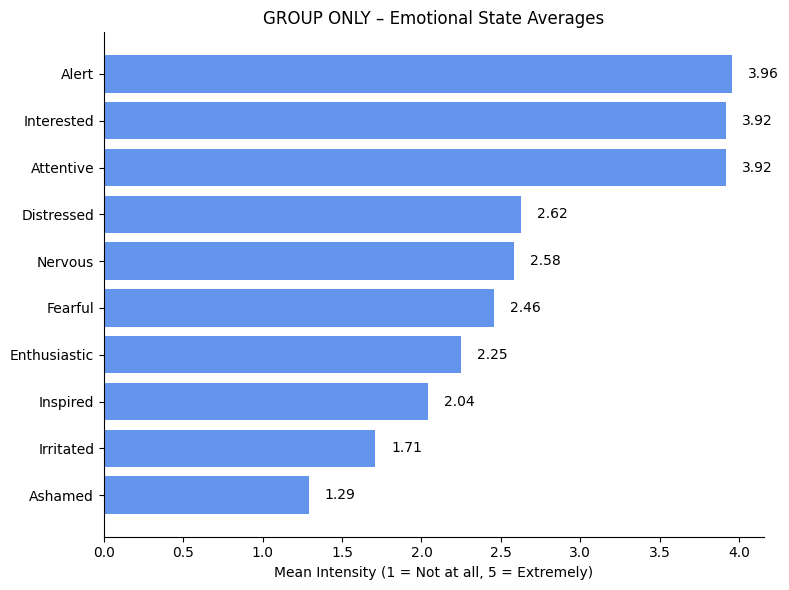
\includegraphics[width=0.75\textwidth]{../../Figures/emotional-post-grp.png}
    \caption{Average emotional state ratings – Group participants only.}
    \label{fig:emotional_post_group}
\end{figure}

As shown in Figure~\ref{fig:emotional_post_group}, \textit{Alert}, \textit{Interested}, and \textit{Attentive} again appeared most strongly. The spread of emotional intensities was relatively consistent with the full group.

The distribution of their overall empathy scores is presented below.

\begin{figure}[H]
    \centering
    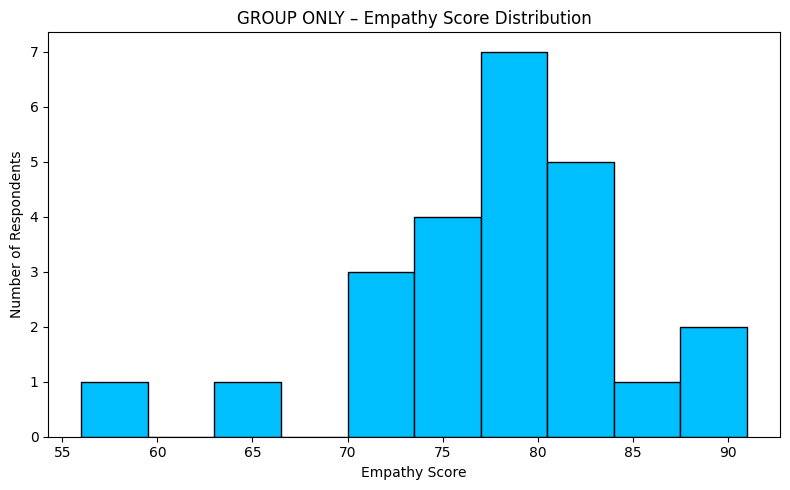
\includegraphics[width=0.75\textwidth]{../../Figures/empathy-score-post-grp.png}
    \caption{Empathy score distribution – Group participants only.}
    \label{fig:empathy_group_post}
\end{figure}

The majority of participants in the group condition scored between 75 and 85 on the empathy scale (max = 91), indicating high levels of empathy across the group.

\subsection{Individual Participants – MR Headset Users}

Participants who engaged with the MR simulation individually using the headset demonstrated slightly different patterns. Their emotional responses included relatively higher levels of \textit{Distress} and \textit{Nervousness}, suggesting a deeper affective impact.

\begin{figure}[H]
    \centering
    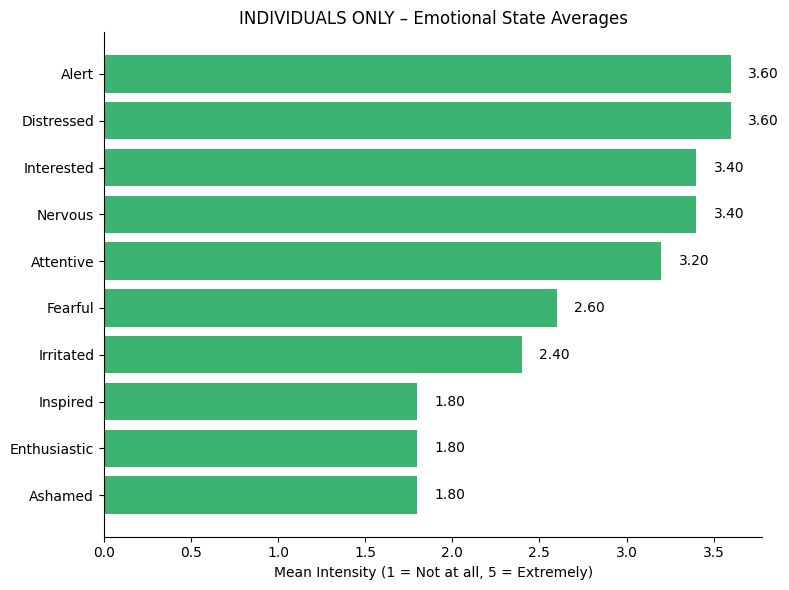
\includegraphics[width=0.75\textwidth]{../../Figures/emotional-post-indiv.png}
    \caption{Average emotional state ratings – Individual (headset) participants.}
    \label{fig:emotional_post_indiv}
\end{figure}

While cognitive engagement emotions like \textit{Alert} and \textit{Interested} remained high, headset users also showed increased ratings for affective states such as \textit{Distressed}, \textit{Fearful}, and \textit{Nervous}, suggesting that the immersive simulation may have elicited stronger emotional reactions.

\begin{figure}[H]
    \centering
    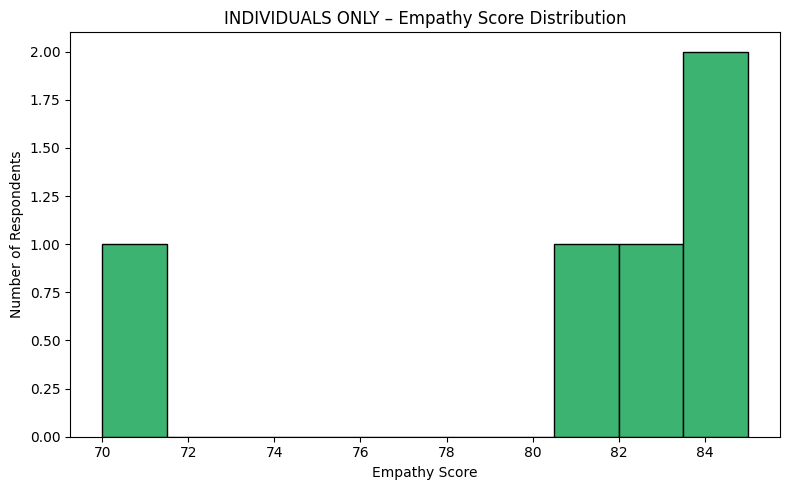
\includegraphics[width=0.75\textwidth]{../../Figures/empathy-score-post-indiv.png}
    \caption{Empathy score distribution – Individual (headset) participants.}
    \label{fig:empathy_indiv_post}
\end{figure}

Empathy scores in this group were tightly clustered at the higher end of the scale, indicating that most headset users reported strong empathic attitudes following the simulation.

\subsection{Overall Empathy Score Distribution}

The full sample distribution of post-evaluation empathy scores is shown below. The majority of respondents scored between 75 and 85 out of 91, reflecting high baseline and post-intervention empathy.

\begin{figure}[H]
    \centering
    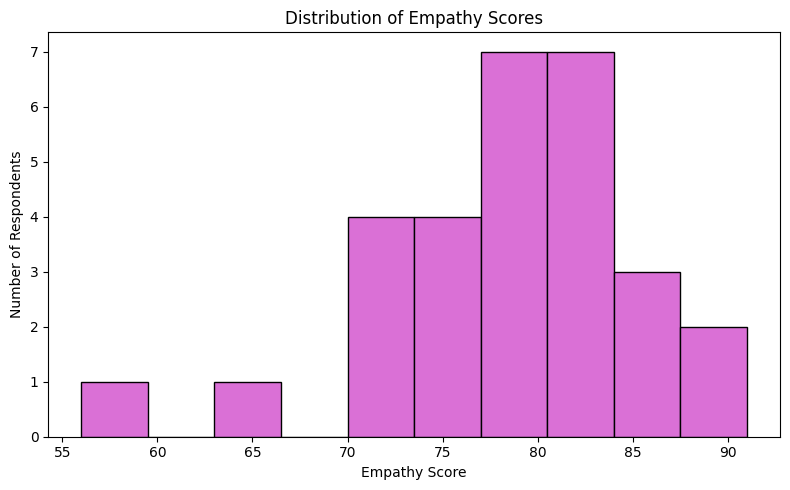
\includegraphics[width=0.75\textwidth]{../../Figures/empathy-score-post-all.png}
    \caption{Empathy score distribution – All participants.}
    \label{fig:empathy_all_post}
\end{figure}

\subsection{Simulation Evaluation Statements}

Participants were also asked to rate their agreement with various statements evaluating the simulation experience. These were scored on a 7-point scale (1 = Strongly Disagree, 7 = Strongly Agree).

\begin{figure}[H]
    \centering
    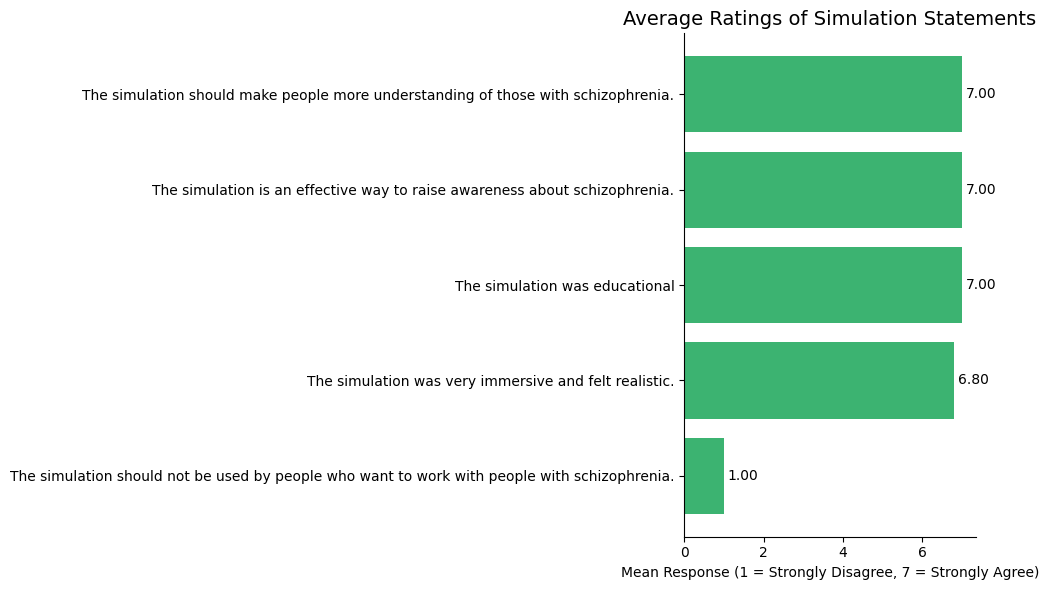
\includegraphics[width=0.9\textwidth]{../../Figures/simulation-evaluation-post.png}
    \caption{Average participant ratings of simulation statements.}
    \label{fig:simulation_evaluation_post}
\end{figure}

Figure~\ref{fig:simulation_evaluation_post} shows near-universal agreement on the simulation’s educational value, realism, and ability to foster understanding. The only statement that received strong disagreement was the suggestion that the simulation “should not be used by people who want to work with people with schizophrenia,” reflecting strong perceived value and acceptability of the tool.

\section{Pre vs. Post Comparison Analysis}
This section presents a statistical comparison of participants’ empathy and emotional responses before and after the simulation experience. By analyzing both group-level changes and individual-level changes, we evaluate whether the intervention led to measurable shifts in perspective or affect. Empathy scores, cognitive and affective, and emotion ratings were analyzed using methods suited for this data.

\subsection{Score Matching and Methodology}

Empathy scores were calculated based on 13 Likert-style attitude items, some of which were reverse-scored to account for negatively phrased statements. Each participant's total empathy score was the sum of their responses, yielding a possible range of 13 to 91 points.

To evaluate changes in emotional response and empathy after the intervention, we conducted paired comparisons between pre- and post-evaluation data. The primary statistical test which was employed for this is the \textbf{Wilcoxon Signed-Rank Test:} used to assess empathetic and emotion-related changes, due to the ordinal nature of Likert data and lack of distribution assumptions.

All tests were two-tailed with a significance threshold of $p < 0.05$. The Wilcoxon test was chosen over a paired t-test due to the non-normal distribution of the data. This approach is robust for small sample sizes and ordinal data \cite{Wilcoxon2013}.

The hypotheses for this test were defined as follows:

\begin{itemize}
  \item \textbf{Null hypothesis ($H_0$):} There is no difference in median empathy scores between the pre- and post-evaluation.
  \item \textbf{Alternative hypothesis ($H_1$):} There is a difference in median empathy scores between the pre- and post-evaluation.
\end{itemize}


\subsection{Statistical Test Results}

To assess the impact of the intervention, we applied statistical tests to compare pre- and post-evaluation responses. These analyses focused on total empathy scores, cognitive and affective empathy subscores, and emotion ratings, with significance evaluated at $p < 0.05$.


\subsubsection{Empathy Score Comparison}

We compared pre- and post-evaluation empathy scores using a Wilcoxon signed-rank test to assess the effect of the intervention.

\begin{itemize}
  \item \textbf{Mean (Pre-Evaluation):} 78.66
  \item \textbf{Mean (Post-Evaluation):} 78.28
  \item \textbf{Wilcoxon test:} $W = 186.0,\ p = 0.7723$
\end{itemize}

While the mean empathy score decreased slightly from pre to post evaluation, the difference was not statistically significant based on either test. The Wilcoxon test returned a p-value of 0.7723, which is well above the common significance threshold of $\alpha = 0.05$. Therefore, we fail to reject the null hypothesis. While the mean empathy score decreased slightly from pre to post evaluation, the difference was not statistically significant. This suggests that the intervention may not have produced a measurable change in empathy, or that individual effects varied too widely for an overall trend to emerge.


\begin{center}
\begin{tabular}{|c|c|c|}
\hline
\textbf{Metric} & \textbf{Pre} & \textbf{Post} \\
\hline
Mean Score & 78.66 & 78.28 \\
Standard Deviation & 4.44 & 7.07 \\
\hline
\end{tabular}
\end{center}

To further explore the effect of the intervention on participant empathy, we examined both the distribution of empathy scores and individual-level changes from pre- to post-evaluation.

\begin{figure}[htbp]
    \centering
    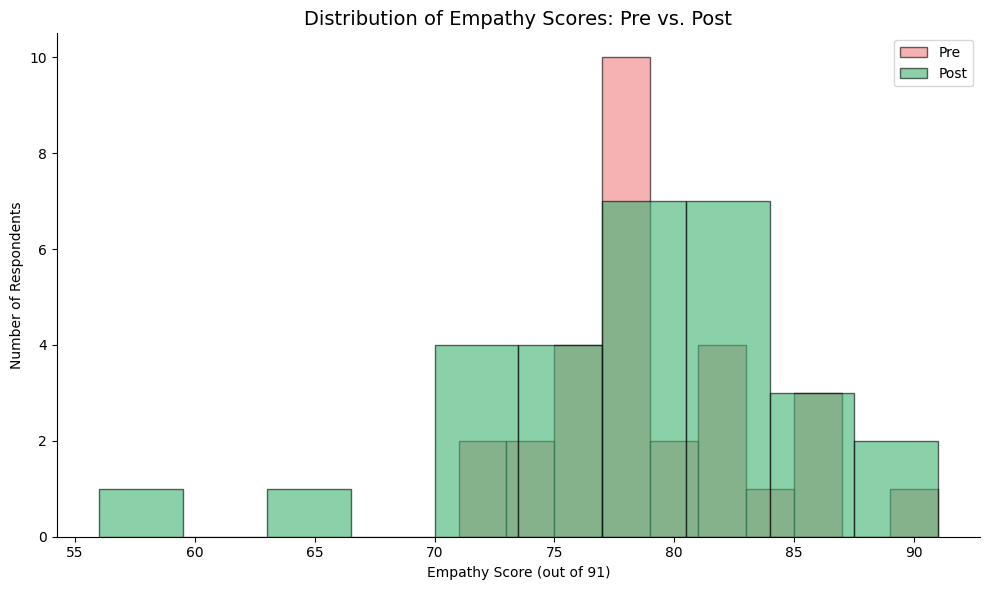
\includegraphics[width=0.75\textwidth]{../../Figures/emp-comparison.png}
    \caption{Distribution of Empathy Scores Before and After the simulation.}
    \label{fig:empathy_dist_hist}
\end{figure}

Figure~\ref{fig:empathy_dist_hist} shows the histogram of empathy scores from the pre- and post-evaluation phases. The distributions are visually similar, with most scores falling between 70 and 85. The post-evaluation scores exhibit slightly more variability, including a small number of lower scores. However, there is also a subtle rightward shift in the upper end, indicating some participants may have increased their scores. Overall, no major distributional shift is apparent.

\begin{figure}[htbp]
    \centering
    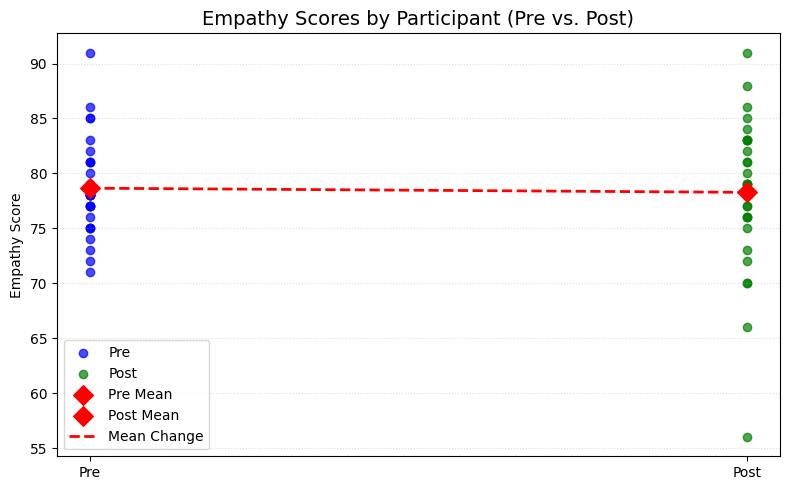
\includegraphics[width=0.75\textwidth]{../../Figures/emph-comparison-means.png}
    \caption{Empathy Scores by Participant: Pre vs. Post with Mean Comparison.}
    \label{fig:empathy_means_line}
\end{figure}

In Figure~\ref{fig:empathy_means_line}, each dot represents a participant’s empathy score before and after the intervention. Red diamonds indicate the group means, and the dashed red line connects the mean pre- and post-scores.

This visualization confirms that although the individual scores are distributed across a similar range, the group mean remained effectively stable. A few participants show noticeable changes in either direction, but the majority maintained consistent empathy scores. The mean dropped slightly from 78.66 (pre) to 78.28 (post), as also reflected in the results of the Wilcoxon signed-rank test ($p = 0.7723$). This supports the interpretation that the intervention did not result in a statistically significant change in overall empathy levels.

These graphs underscore the importance of looking beyond averages: while the group-level effect was minimal, some individuals experienced increases or decreases that could be explored further—especially through qualitative methods or subgroup analysis.

To explore possible group-level effects, we compared average empathy scores by session group. This analysis was motivated by observations made during the simulation sessions: in some groups, the participant using the headset exhibited noticeable engagement — through verbal reactions, physical responses, or expressions of immersion — while in others, the headset user remained relatively passive. Given that the design of the simulation aimed to stimulate empathy through this shared experience, we hypothesized that such variability in engagement might influence group-level outcomes.


\begin{figure}[htbp]
    \centering
    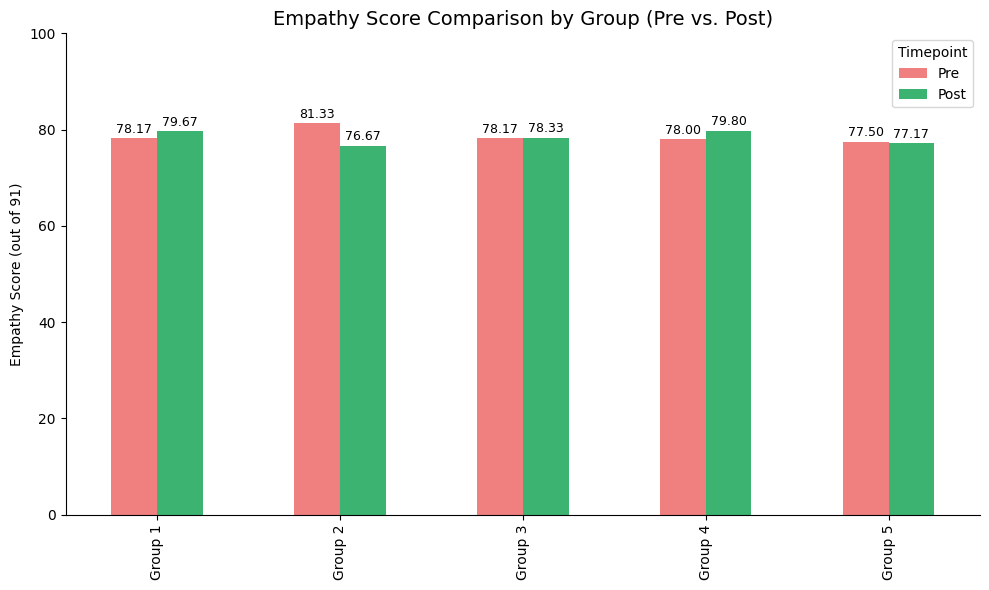
\includegraphics[width=0.85\textwidth]{../../Figures/emph-scores-comp-grp.png}
    \caption{Empathy Score Comparison by Group (Pre vs. Post).}
    \label{fig:empathy_group_bar}
\end{figure}

Figure~\ref{fig:empathy_group_bar} illustrates mean empathy scores for each group before and after the intervention. The scores remain remarkably stable across all groups, with small increases observed in Groups 1, 3, and 4, and small decreases in Groups 2 and 5. None of these differences were large enough to suggest a meaningful group-specific effect. This reinforces the previous conclusion that the intervention did not produce a systematic shift in overall empathy scores.

To better understand the nature of the empathy being measured, we also decomposed the total score into two subcomponents: \textit{cognitive empathy}, which reflects perspective-taking and understanding mental states; and \textit{affective empathy}, which involves emotional resonance and compassion.

\begin{figure}[htbp]
    \centering
    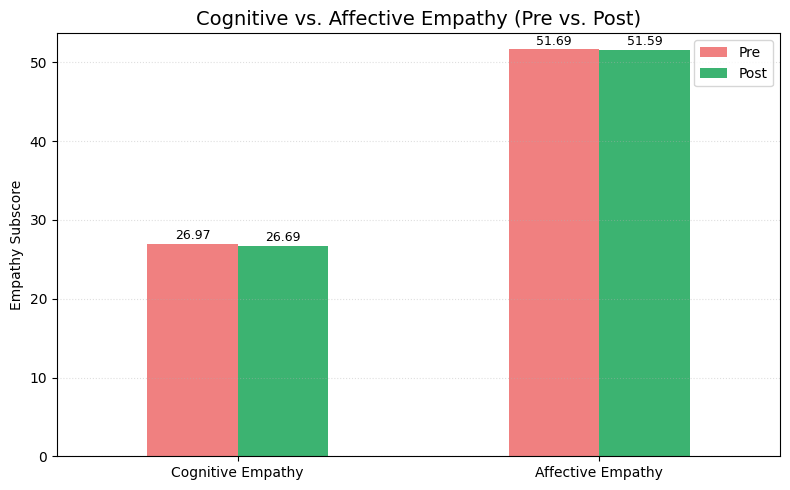
\includegraphics[width=0.75\textwidth]{../../Figures/cog-vs-affect.png}
    \caption{Cognitive vs. Affective Empathy Scores (Pre vs. Post).}
    \label{fig:empathy_cog_aff}
\end{figure}

As shown in Figure~\ref{fig:empathy_cog_aff}, there was almost no change in either subscore. The average cognitive empathy score dropped minimally from 26.97 to 26.69, while the affective empathy score showed an equally small decrease from 51.69 to 51.59. These results suggest that neither cognitive nor affective dimensions of empathy were meaningfully altered by the simulation experience.

Together with the individual, group, and total score analyses, this subscale breakdown adds further support to the interpretation that the intervention had limited impact on participants' self-reported empathy levels — at least as measured immediately after the experience.

% \subsection{Comparison: Individual Headset Users vs. Pre-Evaluation Group}

% To assess whether the most immersive condition—the individual use of the MR headset—was associated with greater empathy, we conducted an exploratory comparison between the post-evaluation scores of headset users ($n=5$) and the pre-evaluation scores of the full participant group ($n=29$).

% The average empathy score for headset users was slightly higher (80.6) than that of the pre-evaluation group (78.7). To test whether this difference was statistically meaningful, we applied the Mann–Whitney U test, a non-parametric method appropriate for comparing two independent groups.

% \begin{itemize}
%   \item \textbf{Mean (Pre-Evaluation Group):} 78.66
%   \item \textbf{Mean (Individual Headset Users):} 80.60
%   \item \textbf{Mann–Whitney U test:} $U = 48.0,\ p = 0.2409$
% \end{itemize}

% As the p-value exceeds the conventional significance threshold of $0.05$, we fail to reject the null hypothesis and conclude that the observed difference is not statistically significant. Nevertheless, the direction of the effect—higher empathy among headset users—may suggest a potential trend.

% \begin{figure}[htbp]
%     \centering
%     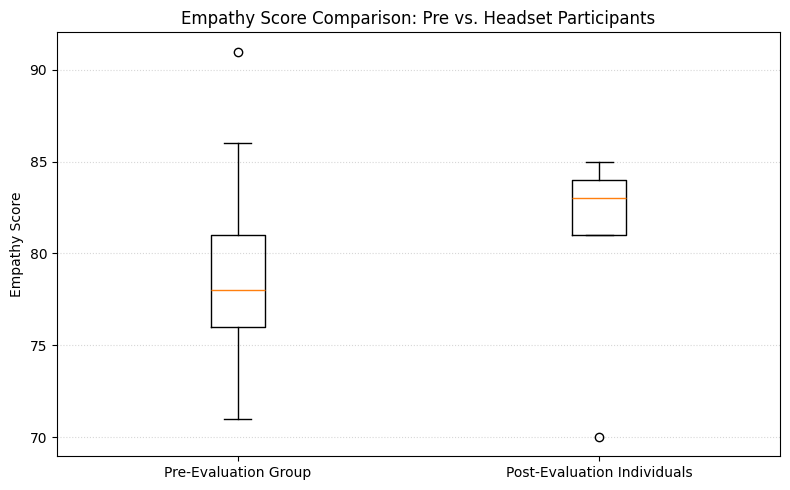
\includegraphics[width=0.75\textwidth]{../../Figures/boxplot-indiv.png} 
%     \caption{Empathy score comparison between individual headset users and pre-evaluation group.}
%     \label{fig:boxplot_indiv_vs_pre}
% \end{figure}

% Given the very small sample size of the individual condition, these results should be interpreted cautiously. However, they offer a potentially meaningful signal: the immersive, embodied experience may have contributed to slightly elevated empathic responses. Future studies should explore this with larger samples and through the integration of qualitative data on individual experiences.


\subsubsection{Emotional Response Comparison}

To explore whether participants’ emotional responses toward people with schizophrenia changed following the simulation, we conducted a series of Wilcoxon signed-rank tests—one for each of the ten emotion items reported pre- and post-intervention.

\paragraph{Hypotheses.} For each emotion, the test was conducted under the following hypotheses:
\begin{itemize}
    \item \textbf{Null Hypothesis ($H_0$):} There is no median difference in emotional intensity pre- and post-simulation; i.e., the simulation did not affect how strongly participants felt the emotion.
    \item \textbf{Alternative Hypothesis ($H_1$):} There is a median difference in emotional intensity between pre- and post-simulation responses.
\end{itemize}

\begin{table}[H]
\centering
\caption{Wilcoxon Signed-Rank Test Results for Emotion Changes}
\begin{tabular}{|l|c|c|c|c|c|}
\hline
\textbf{Emotion} & \textbf{Pre Mean} & \textbf{Post Mean} & \textbf{W-statistic} & \textbf{p-value} & \textbf{Significant} \\
\hline
Attentive     & 4.241 & 3.793 & 72.0  & 0.0633  & False \\
Fearful       & 2.897 & 2.483 & 77.0  & 0.1739  & False \\
Ashamed       & 1.241 & 1.379 & 14.5  & 0.3302  & False \\
Enthusiastic  & 2.379 & 2.172 & 97.5  & 0.3353  & False \\
Nervous       & 2.931 & 2.724 & 86.0  & 0.4702  & False \\
Inspired      & 2.207 & 2.000 & 48.0  & 0.4903  & False \\
Distressed    & 2.621 & 2.793 & 108.0 & 0.5387  & False \\
Irritated     & 1.759 & 1.828 & 47.5  & 0.7483  & False \\
Interested    & 3.862 & 3.828 & 89.5  & 0.8190  & False \\
Alert         & 3.931 & 3.897 & 150.0 & 1.0000  & False \\
\hline
\end{tabular}
\label{tab:wilcoxon_emotions}
\end{table}

None of the tested emotions showed a statistically significant difference between the pre- and post-evaluations at the $p < 0.05$ threshold. The emotion \textit{Attentive} approached significance ($p = 0.0633$), suggesting a possible decrease in attentiveness after the simulation, but this trend did not reach statistical reliability.

To visualize the direction and relative magnitude of changes, the figure below shows the average change in each emotion (post minus pre). Positive values indicate increased emotional intensity post-simulation.


\begin{figure}[H]
    \centering
    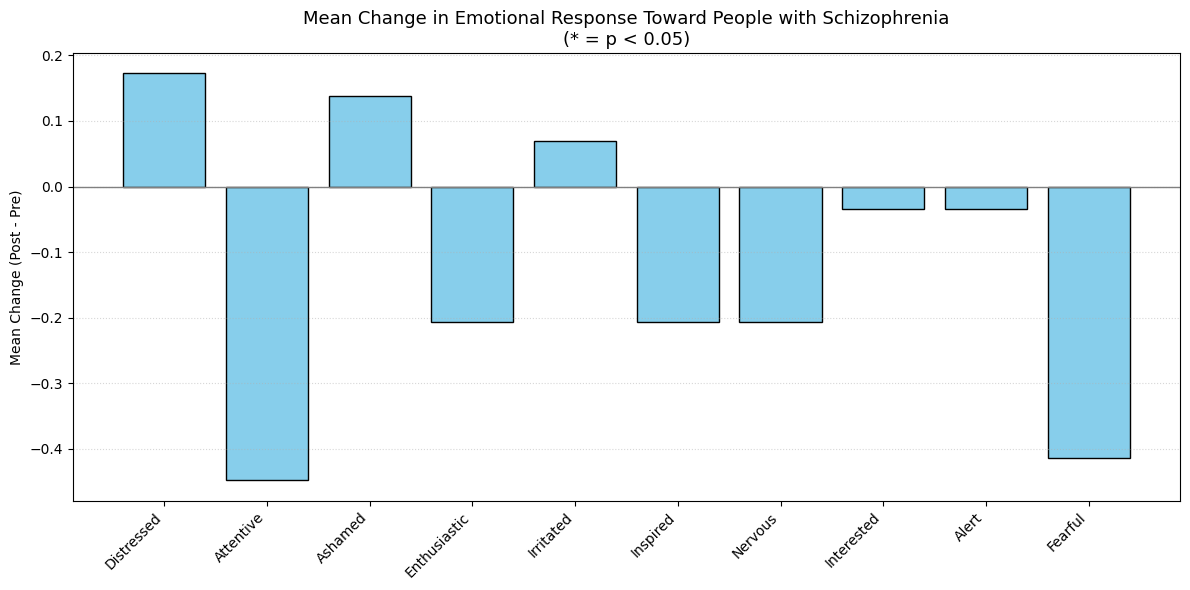
\includegraphics[width=0.85\textwidth]{../../Figures/mean-change-emotions.png}
    \caption{Mean change in emotional response toward individuals with schizophrenia. (* = $p < 0.05$)}
    \label{fig:emotion_change}
\end{figure}

While no statistically significant changes were found, the figure illustrates trends in participants’ emotional shifts. Notably, small increases were observed for emotions like \textit{Distressed}, \textit{Ashamed}, and \textit{Irritated}, whereas emotions such as \textit{Fearful}, \textit{Alert}, and \textit{Attentive} showed modest decreases.

These results suggest that while the simulation may have had subjective effects on emotional perception, the changes were neither strong nor consistent enough to yield significant results across the group. Further qualitative analysis or larger samples may help better characterize individual emotional impacts.


\section{Mixed Methods Integration}
In addition to statistical analyses, observational and self-reported qualitative data were collected to complement the quantitative findings. This included behavioral observations during the MR experience, informal comments post-session, and open-ended feedback where available.

Participants who wore the MR headset shared reflections that contextualized their Likert-scale responses. These insights helped explain individual variability and added depth to our understanding of the simulations emotional impact.


\subsection{Participant Experience and Observational Feedback}

During each session, one participant wore the MR headset simulating auditory and visual hallucinations while attempting to complete a simple task. The rest of the group observed and participated in the same task under normal conditions. This design aimed to allow both the headset user to experience symptoms first-hand and the group to witness their visible effects, ideally fostering empathy through both perspectives.

Notable behavioral patterns varied across participants. Some headset users displayed visible signs of discomfort, such as pinching their lips, turning their heads, hesitating, or seeking clarification. Others remained largely focused on the task, displaying minimal reaction to the simulation.

Group reactions also varied: in some cases, there were uneasy chuckles, concerned glances, or verbal encouragements (“be brave,” “do you need help?”). In other groups, external participants were largely unaware of the internal struggle the headset user was experiencing—sometimes forgetting the headset was even present.

\begin{table}[H]
\centering
\caption{Summary of Headset User Experience and Group Reactions}
\begin{tabular}{|c|p{4.2cm}|p{4.2cm}|p{4.8cm}|}
\hline
\textbf{Group} & \textbf{Headset User Behavior} & \textbf{Group Reaction} & \textbf{Key Participant Quotes} \\
\hline
Group 1 & Nervous laughter, looked around, avoided interacting with virtual elements, reported confusion. & Limited group reaction; one participant quietly offered encouragement. & “The voices keep pulling you down.” \newline “It’s persecution.” \newline “I now understand my cousin better.” \\
\hline
Group 2 & Initially unreactive, later visibly overwhelmed, touched spheres, slight disorientation. & Mild group curiosity, one noted concern, most forgot headset was active. & “There was too much information.” \newline “I forgot the instructions.” \newline “It's harder not to do what the voices say.” \\
\hline
Group 3 & Visibly uncomfortable, delayed task start, repeated lip-pinching, eventually emotional. & Group unaware during task, visibly moved after, discussion emerged post-experience. & “It was horrible.” \newline “I couldn't concentrate... even now I don't know.” \newline “If 2 minutes is absorbing, I can't imagine the people who feel that way every day.” \\
\hline
Group 4 & Focused externally, but no interaction with visual stimuli. Seemed shocked post-experience. & Participant’s distress was internalized; group noticed little during the task. Two members heard audio leaks. & “The voices were disturbing.” \newline “Living the symptoms is another level of experience.” \newline “I think I have more empathy now.” \\

\hline
Group 5 & Started quickly but showed signs of discomfort; pinched lips and waited impatiently for the end. & Group was mostly unaware of the participant’s inner struggle. & “It took a lot of energy and concentration.” \newline “The longer it took, the more frightening it became.” \newline “The simulation helped me realize what they go through.” \\

\hline
\end{tabular}
\label{tab:qual_summary}
\end{table}


\subsubsection{Verbal Feedback from Participants}

Several headset users described strong emotional and cognitive impacts during the debrief. Themes included difficulty concentrating, feeling overwhelmed, dissonance between task instructions and intrusive voices, and a greater understanding of what people with schizophrenia might endure. Some illustrative quotes include:

\begin{itemize}
  \item “We try to focus on something good but the voices keep pulling you down.”
  \item “At first I really didn't want to listen to the voices, but then I couldn't… It's harder not to do what the voices say.”
  \item “I couldn’t understand the instructions… even now I don’t know what we were supposed to do.”
  \item “It was horrible. The voices made simple tasks feel impossible.”
  \item “It was emotionally sad… I didn’t want to look up because I was scared of what I’d see.”
  \item “It took a lot of concentration… I was glad when it was over.”
  \item “I remember my cousin has schizophrenia… now I feel like I better understand what he feels.”
\end{itemize}

Observers also shared reflections:

\begin{itemize}
  \item “I forgot she was wearing the headset… then I saw her moving strangely and I got worried.”
  \item “Seeing her struggle was emotional. It changed how I think about people with schizophrenia.”
  \item “She didn’t react much, so I didn’t realize it was hard for her.”
\end{itemize}

\subsubsection{Interpretation and Reflection}

The qualitative data collected from the debriefs offer valuable insights that contextualize the lack of statistically significant changes in empathy scores. While numeric measures showed minimal change, many participants described deep emotional and cognitive disruption during the simulation, often in ways that are not easily quantifiable.

A consistent theme was the intensity of auditory hallucinations, often overpowering both the visual distortions and the task instructions. Participants reported being distracted, misled, or emotionally shaken. Several remarked on a change in their perspective, noting a greater sense of empathy or awareness after the experience.

Importantly, the visibility of the experience to observers varied greatly. In some groups, the headset users reactions were subtle or absent, making it difficult for others to relate or engage. In others, discomfort or confusion was clearly visible and provoked emotional reactions among the others. This variation highlights the importance of guided debriefs and shared reflection to fully activate the empathy potential of such simulations.

While the intervention may not have uniformly altered self-reported empathy scores, these qualitative accounts suggest that for many participants, the experience was personally impactful—emotionally and cognitively. Future iterations of this intervention may benefit from including structured reflective discussions or journaling to better capture and reinforce these internal shifts.


\section{Summary of Key Findings}

The results of this mixed-methods study suggest that while the MR simulation did not produce statistically significant changes in empathy scores across the entire sample, it nevertheless produced meaningful cognitive and emotional engagement for many participants. Pre-evaluation results indicated that students began the intervention with relatively high levels of empathy and attentiveness, leaving limited room for  movement in quantitative scores—a classic ceiling effect. This was particularly evident in the Jefferson Scale of Empathy (JSE), where most participants scored in the upper range both before and after the simulation.

Post-evaluation data confirmed that self-reported empathy remained largely stable. Neither the total empathy scores nor the subcomponents of cognitive and affective empathy showed significant change following the simulation, and statistical comparisons (Wilcoxon signed-rank test) did not support the hypothesis of a group-level shift. Similarly, emotional affect scores from the B-PANAS showed only modest variation pre- and post-intervention, with none reaching statistical significance. Despite these findings, certain trends were observed, such as a slight decrease in attentiveness and modest increases in distress-related emotions for headset users, hinting at subtle internal shifts not fully captured by the quantitative instruments.

More revealing were the qualitative findings, which offered contextual insight into participants experiences. Headset users frequently described strong emotional reactions to the simulation, including difficulty focusing, feelings of helplessness and emotional discomfort. Many noted that the experience altered how they viewed people living with schizophrenia, leading to greater compassion and understanding. Observers, while less emotionally impacted, also reported increased awareness—particularly when they noticed visible signs of struggle in the headset user.

The simulation was broadly perceived as educational and realistic, with participants agreeing that it helped raise awareness about schizophrenia and could be valuable for those preparing to work in mental health care. In almost all groups, students expressed a desire to reflect more deeply on the experience, particularly during the structured debriefs. These reflections helped surface emotional and empathetic responses that were not always visible in the pre/post metrics but nevertheless shaped their learning.

In summary, the mixed-reality simulation appears to have fulfilled its educational intent by invoking a  personal reflection and generating affective resonance, especially among those who engaged directly with the headset. While the immediate quantitative results were not statistically significant, the qualitative accounts indicate that the simulation meaningfully influenced individual perceptions.